\subsection{Kernel configuration}

\begin{frame}
  \frametitle{Kernel configuration and build system}
  \begin{itemize}
  \item The kernel configuration and build system is based on multiple
    Makefiles
  \item One only interacts with the main \kfile{Makefile}, present at
    the {\bf top directory} of the kernel source tree
  \item The configuration is stored in the \code{.config} file at the
    root of kernel sources
    \begin{itemize}
    \item Simple text file, \code{key=value} style
    \end{itemize}
  \item As options have dependencies, typically never edited by hand,
    but through graphical or text interfaces:
    \begin{itemize}
    \item \code{make xconfig}, \code{make gconfig} (graphical)
    \item \code{make menuconfig}, \code{make nconfig} (text)
    \item You can switch from one to another, they all load/save the
      same \code{.config} file, and show the same set of options
    \end{itemize}
  \end{itemize}
\end{frame}

\begin{frame}
  \frametitle{Kernel or module?}
  \begin{itemize}
  \item The {\bf kernel image} is a {\bf single file}, resulting from
    the linking of all object files that correspond to features
    enabled in the configuration
    \begin{itemize}
    \item This is the file that gets loaded in memory by the
      bootloader
    \item All included features are therefore available as soon as the
      kernel starts, at a time where no filesystem exists
    \end{itemize}
  \item Some features (device drivers, filesystems, etc.) can however
    be compiled as {\bf modules}
    \begin{itemize}
    \item These are {\em plugins} that can be loaded/unloaded dynamically to
      add/remove features to the kernel
    \item Each {\bf module is stored as a separate file in the
        filesystem}, and therefore access to a filesystem is mandatory
      to use modules
    \item This is not possible in the early boot procedure of the
      kernel, because no filesystem is available
    \end{itemize}
  \end{itemize}
\end{frame}

\begin{frame}
  \frametitle{Kernel option dependencies}
  \begin{itemize}
  \item There are dependencies between kernel options
  \item For example, enabling a network driver requires the network
    stack to be enabled
  \item Two types of dependencies
    \begin{itemize}
    \item \code{depends on} dependencies. In this case, option A that
      depends on option B is not visible until option B is enabled
    \item \code{select} dependencies. In this case, with option A
      depending on option B, when option A is enabled, option B is
      automatically enabled
    \end{itemize}
  \end{itemize}
\end{frame}

\begin{frame}
  \frametitle{make menuconfig}
  \begin{columns}
    \column{0.5\textwidth}
    \code{make menuconfig}
    \begin{itemize}
      \item Useful when no graphics are available. Pretty convenient too!
      \item Same interface found in other tools: BusyBox, Buildroot...
      \item Required Debian packages: \code{libncurses-dev}
    \end{itemize}
    \column{0.5\textwidth}
    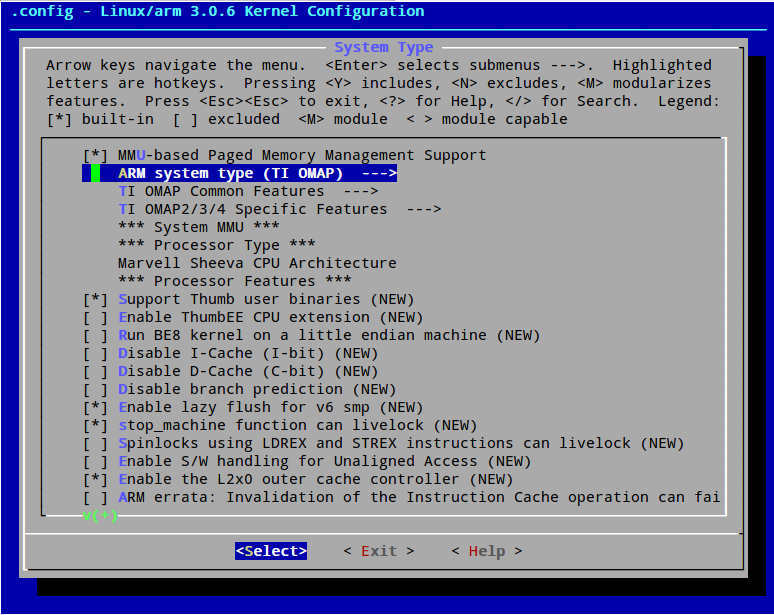
\includegraphics[width=0.9\textwidth]{slides/sysdev-linux-intro-configuration/menuconfig-screenshot.png}
  \end{columns}
\end{frame}

\begin{frame}
  \frametitle{make oldconfig}
  \code{make oldconfig}
  \begin{itemize}
  \item Needed very often!
  \item Useful to upgrade a \code{.config} file from an earlier kernel release
  \item Issues warnings for configuration parameters that no longer
    exist in the new kernel.
  \item Asks for values for new parameters (while \code{xconfig}
    and \code{menuconfig} silently set default values for new
    parameters).
  \end{itemize}
  If you edit a \code{.config} file by hand, it's strongly recommended
  to run \code{make oldconfig} afterwards!
\end{frame}

\begin{frame}
  \frametitle{Undoing configuration changes}
  A frequent problem:
  \begin{itemize}
  \item After changing several kernel configuration settings, your
    kernel no longer works.
  \item If you don't remember all the changes you made,
    you can get back to your previous configuration:\\
    \code{$ cp .config.old .config}
  \item All the configuration interfaces of the kernel
    (\code{xconfig}, \code{menuconfig}, \code{oldconfig}...) keep
    this \code{.config.old} backup copy.
  \end{itemize}
\end{frame}
